\chapter{Literature Review} % Main chapter title

\label{Chapter2} % Change X to a consecutive number; for referencing this chapter elsewhere, use \ref{ChapterX}

\lhead{Chapter 2. \emph{Literature Review}} % Change X to a consecutive number; this is for the header on each page - perhaps a shortened title

The government seems convinced that BIM will solve the problems in the AEC industry through the standardisation of processes and by creating a collaborative culture.
Thus, BIM literature has been reviewed to gain a deeper understanding of BIM, its collaboration-enabling abilities and its adoption in the industry.
%----------------------------------------------------------------------------------------
%	SECTION 1
%----------------------------------------------------------------------------------------

\section{Issues in the Industry}

The AEC industry has recently had a poor reputation due to its poor performance.
An adversarial claims culture emerged within the industry, which often delivered projects that were late, over budget, and of poor quality.
Also, due to a lack of focus on the client, project results tended to drift from the client's original goal.
Hence, this caused an overall dissatisfaction of clients with the AEC industry \citep{lecnotes, Egan1998}.
The poor performance of the industry can largely be attributed to its paradoxical nature; despite the essence of the industry being intense collaborations on bespoke projects in temporary groupings \citep{Laakso2012}, the industry is fragmented, with individual disciplines tending to work in isolation from others \citep{GCS16-20,Miettinen2014}.


%----------------------------------------------------------------------------------------
%	SECTION 2
%----------------------------------------------------------------------------------------

\section{A Call for Collaboration}

In the 1990s, the industry addressed these issues to the UK Government in two key reports: \say{Constructing the Team} by \cite{Latham1994} and \say{Rethinking Construction} by \cite{Egan1998}.
The reports called for a reinvention of the AEC industry to improve its performance and put the client back in the centre.
In order to achieve this, a need for collaboration and standardisation was highlighted.
\cite{Latham1994} and \cite{Egan1998} asked the government to implement their propositions for improvement and to commit itself to becoming a best practice client, thus setting an example for the rest of the industry's clients.


Since then, the government has agreed to become an exemplary client and to implement the reports' propositions.
This is evidenced by a series of documents, including the Government Construction Strategies (GCSs) of 2011-15 by the \cite{GCS11-15} and of 2016-20 by the Infrastructure and Projects Authority \citep{GCS16-20}.
The government's motivations for doing this have been to reduce the cost of its construction projects by up to 20\% and improve the value offered by public sector construction \citep{GCS11-15}.
Amongst the government's strategies for achieving this goal were enabling early contractor and supply chain involvement, standardising products and processes, and replacing adversarial cultures with collaborative ones.
As part of the mobilisation towards collaboration, GCS 2011-15 required Building Information Modelling (BIM) Level 2 as a minimum on all public sector projects by 2016 \citep{GCS11-15}.
Likewise, one of the principal objectives of GCS 2016-20 is to further embed and increase the use of digital technology such as BIM \citep{GCS16-20}.

%----------------------------------------------------------------------------------------
%	SECTION 3
%----------------------------------------------------------------------------------------

\section{BIM} \label{bim}
% Then I'll go on to talk about the facilitators of communication and collaboration. 
% Tools: BIM (Lvl 2 required by 2016 by GCS)
According to the British National Building Specification \citep{NBS2016} and the American National Institute of Building Sciences \citep{NIBSnd}, BIM is the process for creating, managing, and communicating information and knowledge about a built asset throughout its lifecycle, from inception to demolition.
A key output of the process is the building information model (a.k.a. BIM model), a digital file describing every aspect of the built asset.
Overall, literature agrees that the collaborative environment is one of the best aspects of BIM \citep{Santos2017}.
This would explain why the GCSs pushed for the adoption of BIM, believing that it could assist in the reduction of \say{abortive work, discrepancies and mistakes, and inefficiencies in the information supply chain [which] are major contributors to [the industry's] waste} \citep{NBS2014}.

However, the government has recognised that the process of moving the construction industry to `full' collaborative working will be progressive.
Hence, it has defined distinct and recognisable milestones within that process in the form of `levels', as illustrated in Figure \ref{levels}.
Of these levels, the government mandated BIM Level 2 as a minimum on all public sector projects by 2016 \citep{GCS11-15}.
\cite{NBS2014} defines BIM Level 2 as \say{distinguished by collaborative working – all parties use their own 3D CAD models, but not necessarily working on a single, shared model. The collaboration comes in the form of how the information is exchanged between different parties – and is the crucial aspect of this level. Design information is shared through a common file format, which enables any organisation to be able to combine that data with their own in order to make a federated BIM model, and to carry out interrogative checks on it.}

\begin{figure}[htbp]
	\centering
	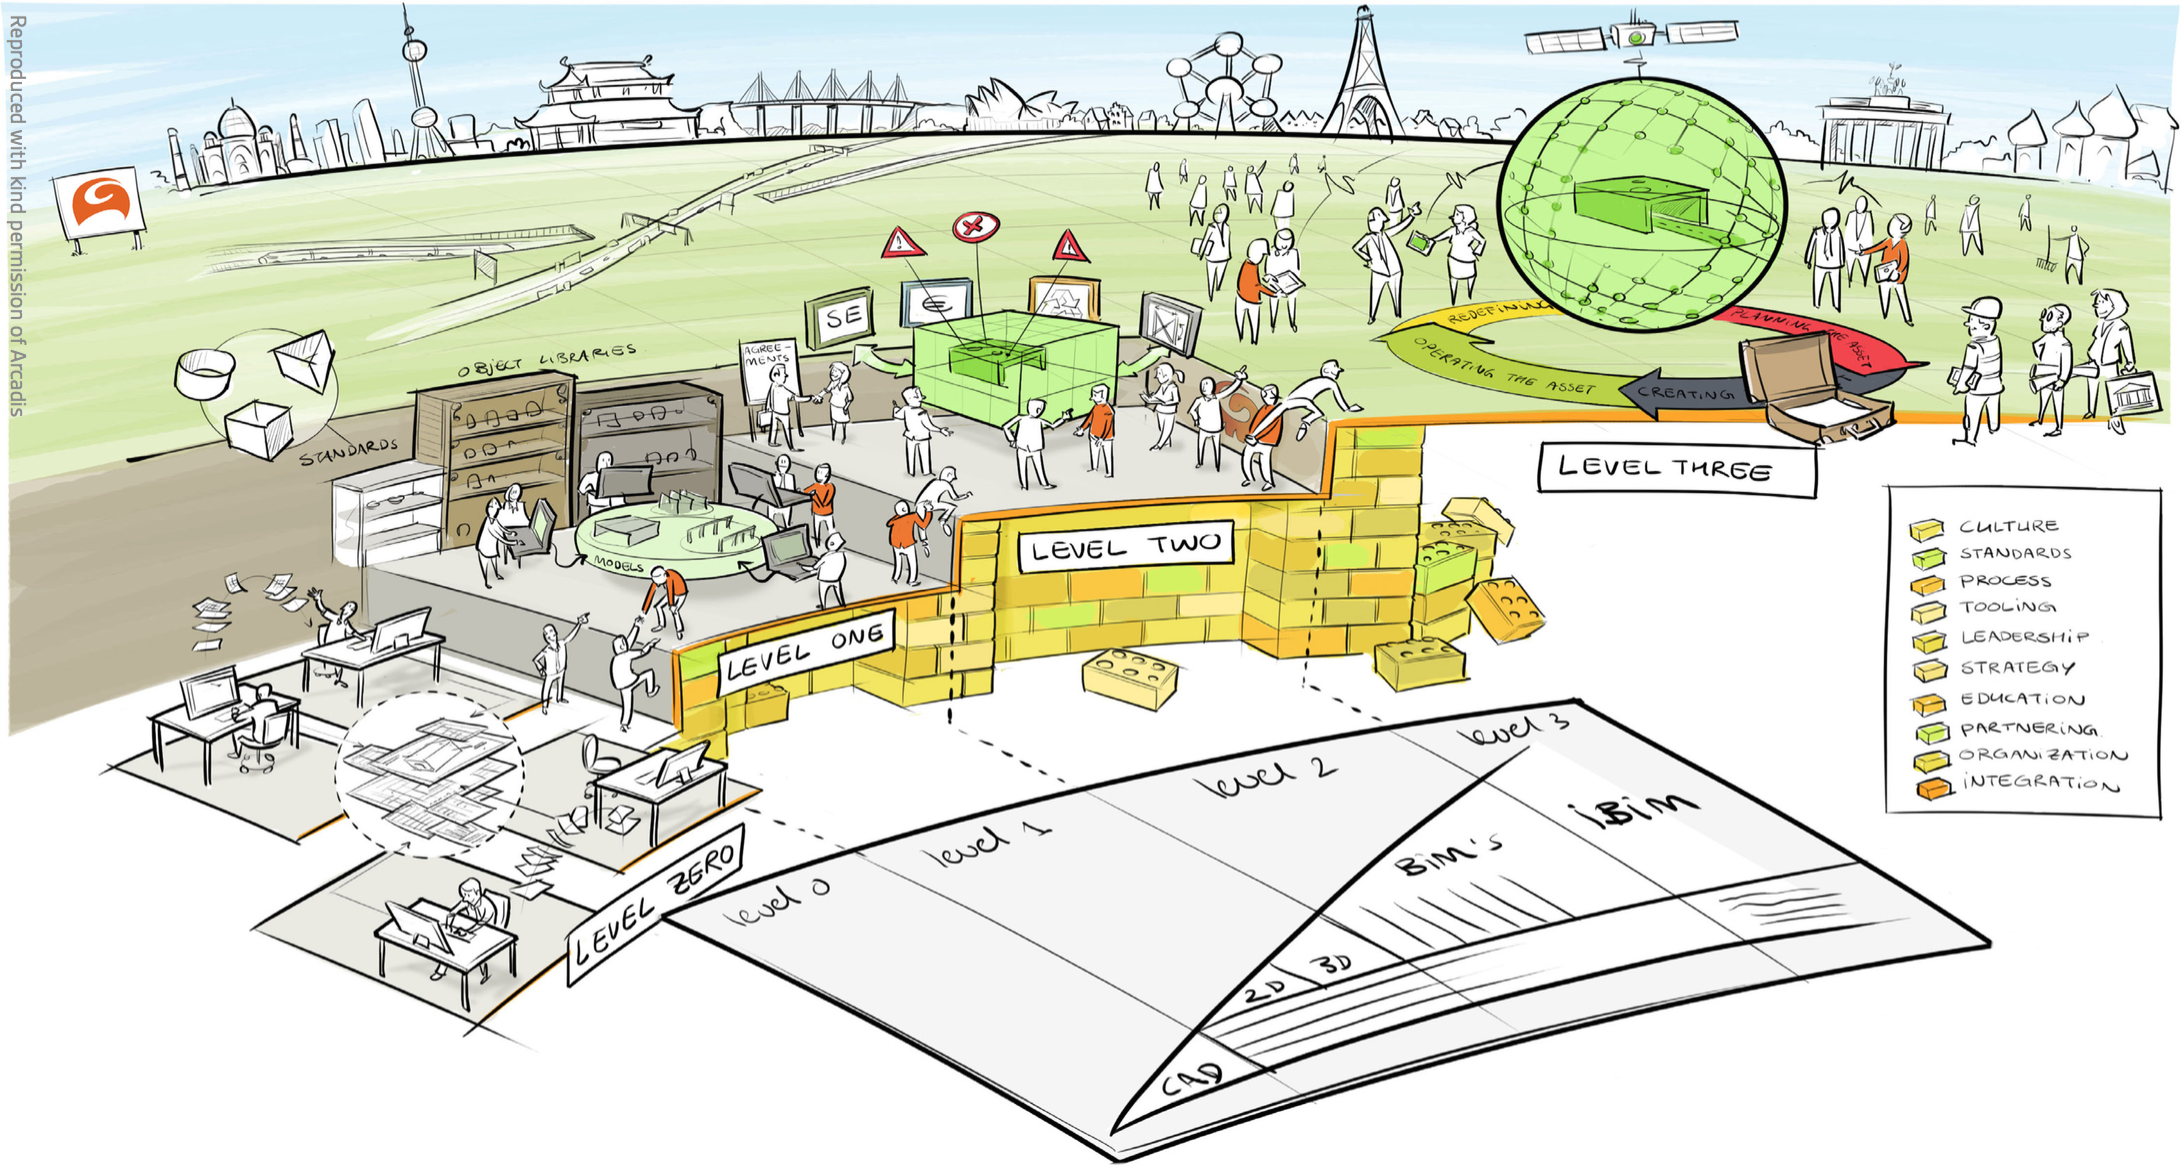
\includegraphics[width=\textwidth]{figures/BIMlevels.png}
	\rule{\textwidth}{0.5pt} % use line???
	\caption[BIM levels]{BIM levels \citep{BSI}.}
	\label{levels}
\end{figure}


As per the government's wish for the standardisation of products and processes, standards have been published and processes established that support the industry's mobilisation towards collaboration.
Processes include the RIBA Plan of Work (PoW) 2013 which \say{provides a framework for the project team to approach design, construction and operational processes} and the BIM Task Group's Digital PoW which \say{aims to provide clarity on how built asset data is defined, tested and successfully used by the supply chain and the public client to achieve BIM Level 2} \citep{Fairhead2015:online}.
Standards have been rapidly developed to meet the immediate market need for BIM Level 2 guidance \citep{NBS2017}.
These rapidly developed standards, a.k.a. Publicly Available Specifications (PAS), and other British Standards (BS) are listed in Figure \ref{stds}.


\begin{figure}[htbp]
	\centering
	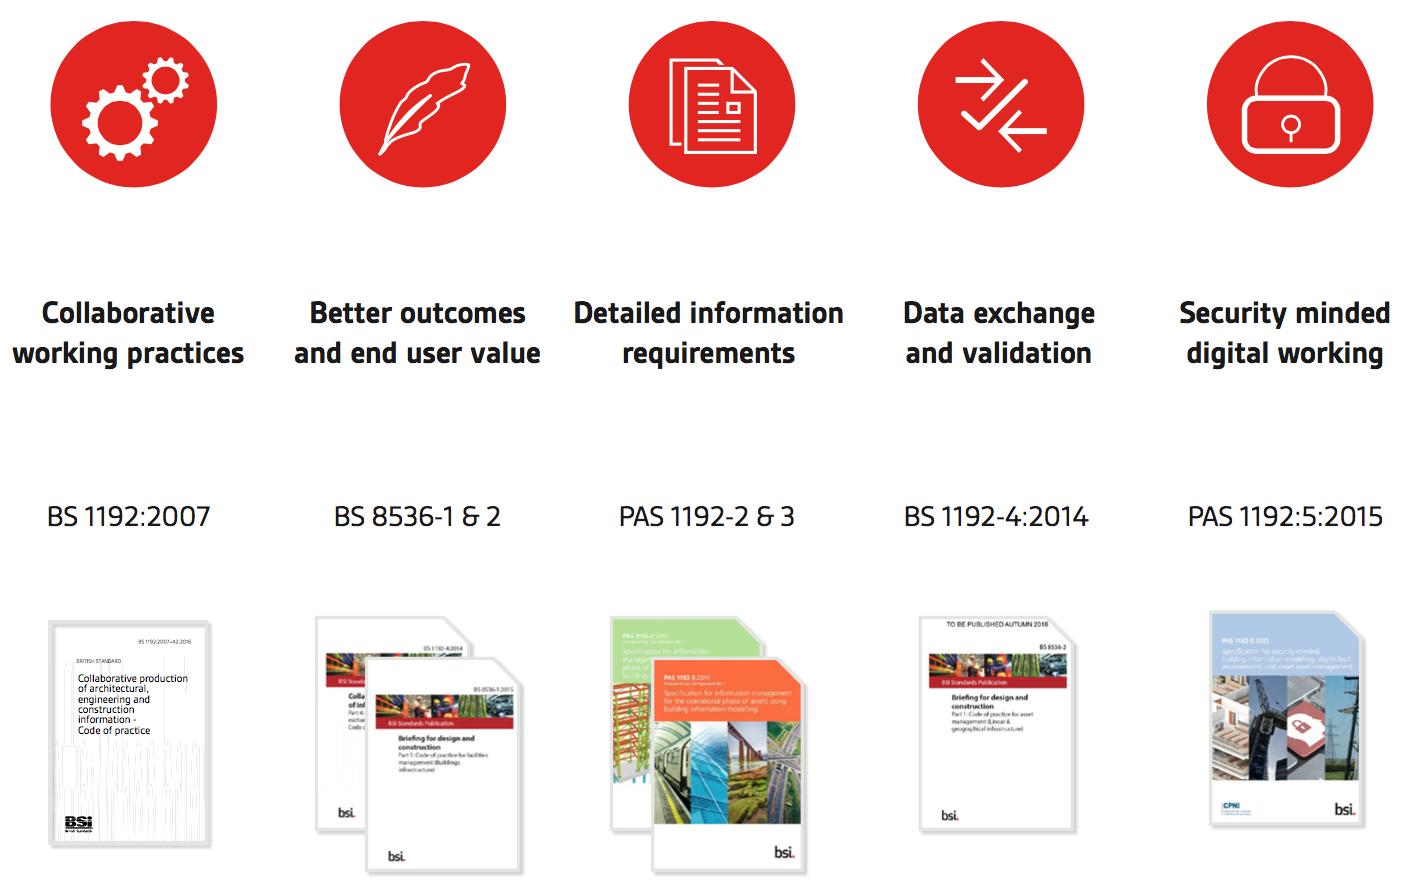
\includegraphics[width=\textwidth]{figures/BIMstandards.png}
	\rule{\textwidth}{0.5pt} % use line???
	\caption[BIM Level 2 British Standards and Publicly Available Specifications]{British Standards (BS) and Publicly Available Specifications (PAS) supporting BIM Level 2 adoption \citep{BSI}.}
	\label{stds}
\end{figure}



%----------------------------------------------------------------------------------------
%	SECTION 4
%----------------------------------------------------------------------------------------

\section{Problems Encountered in the Adoption of BIM}
% After that, the problems faced in the adoption of BIM will be described.
In spite of all the support and protocols, the adoption of BIM has been uneven across the industry.
\cite{DesigningBuildingsLtd2017} suggests that the industry is only helping those at the forefront of BIM adoption get better at it while leaving the rest behind, thus making BIM a specialist subject.

Moving to BIM from pen and paper or computer-aided design (CAD) requires a shift in existing work practices \citep{Singh2011}.
A case study by \cite{Neff2010} gives a couple examples of this shift from the experiences of people in the industry.
Firstly, whereas architects may have appreciated the interpretative flexibility that came with drawings, especially during the conceptual design stages, there is no longer any room for interpretation in BIM models because all the data needs to be inputted exactly.
Secondly, BIM software packages require designers to, for instance, select the colour of a door in the model when it may not yet have been actually decided. 
If the designer were to show that model to the client, the client may get distracted, confused or misled by this `pre-decision'.
Therefore, this over-determination of information that BIM software packages sometimes require can alter or even degrade communication between stakeholders.

Literature shows that there is a reluctance, and sometimes inability, to change existing work practices in order to make the BIM shift.
On the one hand, \cite{Laakso2012} suggest that small companies may not have the resources to adopt BIM.
On the other hand, \cite{Singh2011} suggest that the industry can often find itself stuck in a status quo loop, as illustrated in Figure \ref{loop}.
\say{The lack of knowledge and awareness about BIM can result in a lack of confidence and motivation to adopt BIM-based collaboration. Conversely, as a result of the inhibition to adopt and use BIM, the level of knowledge about BIM remains} \citep[p.~136]{Singh2011}.

\begin{figure}[htbp]
	\centering
	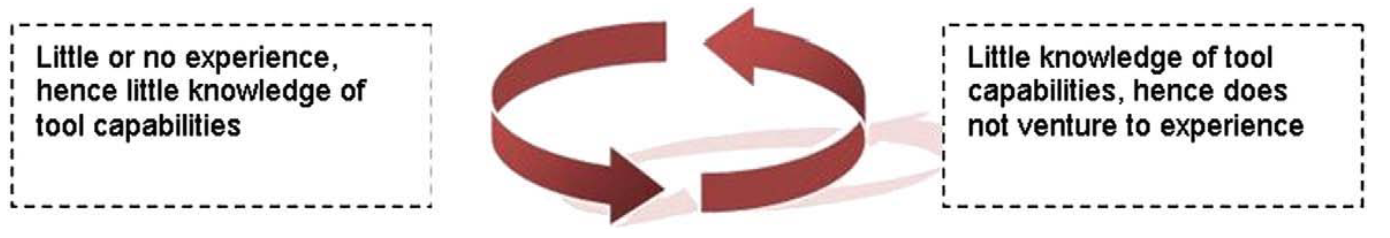
\includegraphics[width=\textwidth]{figures/Loop.png}
	\rule{\textwidth}{0.5pt} % use line???
	\caption[Status quo loop inhibiting BIM adoption]{Status quo loop inhibiting BIM adoption \citep[p.~136]{Singh2011}.}
	\label{loop}
\end{figure}

\noindent
Some other factors that are impeding the adoption of BIM are:
\begin{itemize}
	\item The fragmented nature of the industry \citep{Singh2011,Neff2010} 
	\item A lack of initiative, training and available skilled personnel in BIM \citep{Singh2011,Ghaffarianhoseini2017}
	\item A lack of clarity on roles, responsibilities, and distribution of benefits in adopting the BIM approach \citep{Singh2011,Ghaffarianhoseini2017}
	\item Intellectual property and security-related concerns \citep{Ghaffarianhoseini2017,Laakso2012} 
	\item A lack of interoperability between different pieces of software \citep{GCS11-15,Laakso2012}. 
	(Interoperability is the ability of different software applications to exchange and make use of data \citep{Gallaher2004}.)
\end{itemize}


%------------------------------
%	SUBSECTION 1
%------------------------------

\subsection{A More Realistic View on the Adoption of BIM}
% More sober view of BIM adoption
\cite{Miettinen2014} argue that the industry's expectations of BIM are too high and that the encountered problems are normal in the adoption of a new technology that fundamentally changes how the industry works.
In literature, \cite{Miettinen2014} found a couple reasons for these high expectations.
The first reason is that the promises of the benefits of BIM were initially set high in order to attract financial sponsors and stimulate political agendas.
The second is that there has been a tendency to equate the technological potential of BIM to future reality while ignoring the actual circumstances that are likely to complicate and delay the realisation of that vision.
In fact, \cite{Miettinen2014} claim that it normally takes a company two decades for it to embed a new technology into its work practice from the time the technology is introduced to the company.
% So maybe…


%----------------------------------------------------------------------------------------
%	SECTION 5
%----------------------------------------------------------------------------------------


















\begin{comment}

% CONSTRUCTION INDUSTRY PROBLEMS
The construction industry is highly fragmented \citep{GCS16-20}. 
The construction industry has long been infamous for delivering projects late, over budget or of poor quality. This led to an increase of dissatisfied clients and created an adversarial "claims" culture in the industry. Project outcomes drifted from the original goals due to a lack of focus on the client, poorly defined procurement routes, and contract forms that did not encourage or accommodate colaboration.  (P\&C lec notes)
there is deep concern that the industry as a whole is under-achieving.It has low profitability and invests too little in capital, research and development and training. Too many of the industry's clients are dissatisfied with its overall performance \citep{Egan1998}.


% INDUSTRY TO GOVT: NEED FOR COLLABORATION
Two key joint industry (?) and government reports were published in response to these issues: \say{Constructing the Team} by \cite{Latham1994} and \say{Rethinking Construction} by \cite{Egan1998}. As the reports' titles suggest, these reports called for collaboration and innovation in the construction industry.
\cite{Egan1998} identified five key drivers for change for the industry, one of which was \say{integrated process and teams}. Moreover, \cite{Egan1998} called for standardisation of components and processes in order to \say{design projects for ease of construction}.
Similarly, \cite{Latham1994} called for standardisation by urging clients to start using the New Engineering Contract (NEC) and \say{phase out \say{bespoke} documents}.
Furthermore, both reports asked the government to commit itself to becoming a best practice client and to lead public sector bodies to becoming best practice clients by implementing the reports' propositions and thus setting an example for the rest of the construction industry clients.

% GOVT TO INDUSTRY: OK --> CONDENSE TO 1 PARAGRAPH
The government has since taken action/ responded to the Latham and Egan reports.
The government has published a series of documents with a plan of action of how it and public sector bodies plan to implement Latham's and Egan's propositions, including the Government Construction Strategies (GCS) of 2011-15 \citep{GCS11-15} and 2016-20 \citep{GCS16-20}.
In both of the documents mentioned, the government agrees to become an exemplary client across the industry.

With the ultimate aim of reducing the cost of government construction projects by 15-20\%, GCS 2011-15 identified the need to improve the value offered by public sector construction.
Amongst the strategies of achieving this goal was the promotion of product standardisation and collaborative cultures to replace adversarial ones.
As part of the boration, the report introduced Building Information Modelling (BIM) as offering a \say{a fully collaborative 3D environment, [where] all of those involved in a project are working on a shared platform with reduced transaction costs and less opportunity for error} \citep[p.~13]{GCS11-15}.
Literature supports this, saying that the collaborative environment is one of the best aspects of BIM \citep{Santos2017}.
The report then goes on to say that the \say{Cabinet Office will co-ordinate Government's drive to the development of standards enabling all members of the supply chain to work collaboratively through Building Information Modelling (BIM)}, and that \say{Government will require fully collaborative 3D BIM (with all project and asset information, documentation and data being electronic) as a minimum by 2016} \citep[pp.~13-14]{GCS11-15}.

According to GCS 2016-20, £3 million of efficiency savings were delivered over 2011-15, which was partially enabled by \say{developing new models and approaches to procurement, which focus on collaboration and early contractor involvement} and \say{developing digital capability in design and construction, with all departments on target to procure assets using Building Information Modelling (BIM) Level 2 by 2016} \citep[p.~3]{GCS16-20}.
Following that, two of the four principal objectives of GCS 2016-20 are to (1) embed and increase the use of digital technology, including BIM Level 2, and (2) deploy collaborative procurement techniques that, amongst other objectives, enable early contractor and supply chain involvement \citep[p.~2]{GCS16-20}.

% STDISATION
Compatible tools are vital in an industry such as the construction industry, where several organisations collaborate intensively on bespoke projects in temporary groupings \citep{Laakso2012}.
The best solution would be to have widely accepted and mature technical platforms based on open standards to enable communication and collaboration among project participants without requiring them to have specific proprietary applications.
\say{IFC (Industry Foundation Classes) is an open and standardized data model intended to enable interoperability between building information modeling software applications in the AEC/FM industry} \citep{Laakso2012}. % simpler explanation?
IFC was developed by buildingSMART, formerly known as the IAI (International Alliance for Interoperability).
Although IFC has been around for a long time, even being implemented into leading BIM software, actual use of IFC as an enabler of interoperability has remained low.
Currently, the exchange of BIM data is dominated by proprietary solutions, despite the fact that the industry has been working on specifications for an open data format relatively early with regard to the technological maturity of BIM software.

Two commonly reported interdependent hurdles for achieving the interoperability of integrated BIM within the construction industry have been the fragmented industry actor landscape and the heterogeneous adoption of IT among these actors.
They highlighted how a \say{lack of compatible systems, standards and protocols [has] inhibited widespread adoption of} BIM \citep[p.~13]{GCS11-15}.
Interoperability is not the only culprit in preventing the widespread adoption of collaborative technologies such as BIM, but so are companies' reluctance to share business intelligence or their desire to protect intellectual property etc.

BIM is more than just 3D modeling, it is an integrated semantic/ intelligent product and process model.

Interoperability is the ability to manage and communicate electronic product and project data between collaborating firms and within individual companies' design, construction, maintenance, and business process systems (Gallaher & Chapman 2004).
The benefit of interoperability is illustrated in figure \ref{io}. If no common open standard exists, each individual software application must develop and implement direct translators back and forth for all other pieces of software which it seeks to communicate with. If an open standard can be used instead, the mappings only need to be translated back and forth from that single format in order to be compatible with all other applications supporting the same standard.
Insufficient interoperability can cost money! The United States Institute of Standards (NIST) estimated that it can cost the industry USD 15.8 billion annually. Hence, studies suggest that interoperability can offer considerable finanical savings.
Considering the theoretical benefits of open format, it might seem natural for a user to adopt an open alternative. But, as an anecdotal example shows, this is not always the case. Free and open word processing softwares have been available for several years, and yet Microsoft Word file format (which is a vendor-specific proprietary format) continues to be perceived as the de-facto standard format.




% PROBLEMS


% BIM ADOPTION NOT SO STRAIGHTFORWARD


% 2005-2015 BIM LIT REV
\cite{Santos2017} reviewed a decade of BIM literature (2005-2015). Firstly, they found that Collaborative Environments and Interoperability was currently the most popular area of research. Interestingly they point out that although the collaborative environment is referred to as one of the best aspects of BIM, there are a seemingly low volume of papers addressing the topic.
% I think I may find this area interesting to research, perhaps more specifically collaborative-based platforms/ networks. However, the existing literature in this area (listed below) seems a bit technical, perhaps beyond my scope of capabilities/ knowledge.
% Upon thinking of BIM, I often came across the need for standardisation. With this being related to the ability to communicate and collaborate across different disciplines, platforms, and countries etc., I think standardisation is another interesting topic to look into.
Secondly, they found that BIM Adoption and Standardisation was the category with the third highest number of published papers, being an area that has been explored since the early phases of BIM research. However, there were only a few papers studying and comparing existing BIM standards and protocols. They deduced that there had been a lack of interest in harmonising BIM standards, despite the industry becoming more globalised. Moreover, they found \say{a gap in the literature with regard to the assessment of BIM adoption in a whole region (e.g. at the European level)}.


% BJÖRK: EXPERTS' VIEW ON STDISATION
According to \cite{Santos2017}, one of the first papers on the standardisation of BIM was written by \cite{Howard2008}.
According to \cite{Howard2008}, standards may apply to language, products, elements, or processes.
Their study showed that standards are generally supported and most effective nationally.
However, in order for IFC standards to gain wide recognition and successful implementation, they require international endorsement and formalisation, such as from ISO (International Organisation for Standardisation).


% BEYOND BIM UTOPIA
A position paper by \cite{Miettinen2014} suggested that the industry’s promises of BIM use were but a chimera and proposed more realistic predictions of the development and implementation of BIM.
Firstly, they clarify that there is no single definition for BIM since it is a transdiscursive term used by several disciplines (e.g. research, policy making, and industry) and thus it should be treated as a \say{multidimensional, historically evolving, complex phenomenon}.
Secondly, they identify the source of the wishful thinking and unrealistic promises associated with BIM; \say{(Brown et al. [2000], p.881): Initial promises are set high in order to attract attention from (financial) sponsors, to stimulate agenda setting (both technical and political) [etc.]}.
Another source is the tendency to equate technological potential to future reality while disregarding many of the conditions and constraints that in reality would complicate and retard the realisation of the vision.
\cite{Miettinen2014} listed the four elements of the BIM utopia:
\begin{enumerate}
\item All relevant information will be included in a single BIM;
\item BIM will become a tool of collaboration thanks to the development of standards and interoperability;
\item BIM will be maintained and used throughout a building’s lifecycle;
\item BIM will significantly improve the efficiency and productivity of the industry.
\end{enumerate}

They challenged these visionary elements with actual occurrences.
At the time, BIM tended not to be used exclusively, but as part of \say{hybrid practices}. 
This is partly because some people (e.g. facilities managers) mistrusted BIMs because of the known challenges in updating models, an activity which normally ended during the construction stage. 
Moreover, BIM had not changed tendencies of working in disciplinary \say{silos}, and it was difficult to isolate and evaluate the value of BIM. 
One realistic solution they suggested was introducing \say{knots}, short periods of collaboration where the entire project team met up before splitting up again to work in their \say{silos}.

\cite{Miettinen2014} proposed two approaches to view the implementation of BIM. 
The first was the normative approach that relies on guidelines, training, and presentations of successful cases of BIM use, but which they felt was incomplete and in need of a more realistic complementary view. 
The second was the activity theoretical approach which considers the time and effort required before there is any noticeable increase in productivity. 
This probably involves the re-working of BIM systems to customise them to a company’s needs, which designers may not have anticipated in the development of the technology. 
This approach also suggested a time lag of normally two decades between the time a technology is introduced to a company that is working in a previous paradigm and the time new social and institutional arrangements start to take shape. 
They offered three foreseeable outcomes of the activity theoretical approach:
\begin{enumerate}
\item BIM will be an open-ended expansive process of which the future is unpredictable and unexpected;
\item Multiple solutions will persist despite efforts to standardise;
\item Learning will be by experimentation and invention of novel uses where practitioners and users play a key role.
\end{enumerate}


% THEORETICAL FRAMEWORK (NOT PEER REVIEWED?)
According to \cite{Singh2011}, expectations of BIM varied across disciplines.
Designers viewed BIM as an extension to CAD, whereas non-designers (e.g. contractors and project managers) viewed it as an intelligent document management system.


\end{comment}
